\subsection{Convergence}

In a first step extensive convergence studies are carried out. Therefore, only the elastic part of the material behavior is considered. The load-displacement curves of the PD simulations are compared to the solution obtained by the implicit nonlinear solution in the commercial finite element solver Abaqus. Identical meshes are used in both cases. Using the versatile parametric model generator, the identical discretizations are written for Peridigm and Abaqus.

The stiffness convergence is evaluated by means of the load-displacement behavior. Two aspects of convergence are considered. At first it is investigated if the load-displacement curves asymptotically approach a common course. On the other hand, the load-displacement curve from the local FE solution obtained with Abaqus is used as a second convergence criterion for this simple one-dimensional loading condition. It is not expected that the PD solution must necessarily exactly coincide with the FE result. But for this simple test, large deviations should also not occur in the elastic regime of the material response.

\subsubsection{Hex mesh}

\paragraph{Stiffness}

\autoref{fig:Results:Hex:FD0-4} shows the respective results for an element edge length $dx$ of $\SI{0.4}{\milli\meter}$ and a structured mesh for different horizons. This element edge length is defined over the thickness of the specimen. Due to the dimensions from \autoref{tab:AdhMatChar_ep_BulkTension_Dims}, the in-plane element edge length is $\SI{0.395}{\milli\meter}$ in $x$- and $\SI{0.357}{\milli\meter}$ in $y$-direction. In this study, the horizon is specified by means of an absolute value as proposed by \cite{HuW2012,SaregoG2016} to be able to directly compare the behavior between different element edge length. The non-continuous curves for the PD results are caused by small oscillation in the explicit solution in Peridigm without any damping and a small number of output time steps.

\pgfplotstableread[col sep=comma]{../../Material/Data/Numerics/Hex_0-4_ForceDisplacement.csv}{\loadedtable}

\begin{figure}[htbp]
\centering
\tikzexternalenable
\tikzsetnextfilename{Hex_0-4_ForceDisplacement}
\begin{tikzpicture}
  \setlength{\figheight}{7cm}
  \begin{axis}[
    %height=\figheight+\baselineskip,
    height=\figheight,
    width=0.7\linewidth,
    axis lines=middle,
    cycle list name=color list,%linestyles*,
    xmax=0.5,
    title=\empty,
    xlabel={Displacement $[\si{\milli\meter}]$},
    ylabel={Force $[\si{\newton}]$},
    x label style={at={(axis description cs:0.5,-0.075)},anchor=north},
    y label style={at={(axis description cs:-0.085,.5)},rotate=90,anchor=south},
    legend pos=north west,
    legend cell align={left},
    legend style={font=\footnotesize},
    %scaled x ticks=false,
    xticklabel style={/pgf/number format/fixed},
  ]
    \addplot+ [thick] table[x=DxAbq, y=FxAbq] {\loadedtable};
    \addlegendentry{Abaqus}
    \addplot+ [] table[x=Dx5, y=Fx5] {\loadedtable};
    \addlegendentry{$\delta=\SI{5}{\milli\meter}$}
    \addplot+ [] table[x=Dx4, y=Fx4] {\loadedtable};
    \addlegendentry{$\delta=\SI{4}{\milli\meter}$}
    \addplot+ [] table[x=Dx3, y=Fx3] {\loadedtable};
    \addlegendentry{$\delta=\SI{3}{\milli\meter}$}
    \addplot+ [] table[x=Dx2, y=Fx2] {\loadedtable};
    \addlegendentry{$\delta=\SI{2}{\milli\meter}$}
    \addplot+ [] table[x=Dx1.5, y=Fx1.5] {\loadedtable};
    \addlegendentry{$\delta=\SI{1.5}{\milli\meter}$}
    \addplot+ [] table[x=Dx1.25, y=Fx1.25] {\loadedtable};
    \addlegendentry{$\delta=\SI{1.25}{\milli\meter}$}
    \addplot+ [] table[x=Dx1.2, y=Fx1.2] {\loadedtable};
    \addlegendentry{$\delta=\SI{1.2}{\milli\meter}$}
    \addplot+ [] table[x=Dx1.18, y=Fx1.18] {\loadedtable};
    \addlegendentry{$\delta=\SI{1.18}{\milli\meter}$}
    \addplot+ [] table[x=Dx1, y=Fx1] {\loadedtable};
    \addlegendentry{$\delta=\SI{1}{\milli\meter}$}
    \addplot+ [] table[x=Dx0.875, y=Fx0.875] {\loadedtable};
    \addlegendentry{$\delta=\SI{0.875}{\milli\meter}$}
  \end{axis}
\end{tikzpicture}
\tikzexternaldisable
\caption{Force-displacement plot in elastic region for hex-mesh with $dx=\SI{0.4}{\milli\meter}$ and various horizons}
\label{fig:Results:Hex:FD0-4}
\end{figure}

For the chosen element edge length of $dx=\SI{0.4}{\milli\meter}$, the stiffness reduces with decreasing horizon. This finding does not correspond to the results in \cite{MitchellJA2015} where a LPS material model produces a less stiff behavior than expected. The decrease in stiffness is obtained until $m\approx3$, here $m=\num{2.95}$ for a horizon of $\delta=\SI{1.18}{\milli\meter}$. This matches $m_z=\num{2.95}$, $m_y=\num{3.31}$ and $m_x=\num{2.99}$. The converged PD solution matches the FE solution. If the horizon is decreased below this value, the stiffness rises again compared to the FE solution. This may be caused by the fact, that not enough neighboring points interact in the horizon of a single point to depict the correct material behavior in all directions, including transversal contraction.

For element edge length above $\SI{0.4}{\milli\meter}$ and thus five PD collocation points over the specimen thickness, a similar behavior exists with the exception that the local FE solution is never reached. This seems to be the result of the missing surface correction in the chosen LPS material model implementation in Peridigm. For element sizes smaller than $\SI{0.4}{\milli\meter}$ and thus more elements over the specimen thickness a horizon with good agreement can be found for all considered cases.

The results of the study for different element sizes is shown in \autoref{fig:Results:Hex:Convergence}. Since it is impossible to show the load-displacement curves for all combinations in the context of this study, only the relative error of the force at a displacement of $\SI{0.1}{mm}$ in the load introduction region to the FE solution with an element edge length of $\SI{0.2}{\milli\meter}$ is compared. Results in the upper left corner of the figure are not available as the horizon would be smaller than the element size. The smaller the failure of a combination is, the brighter a point is. A white point corresponds to an error of zero. The minimum combination of each element size and horizon is shown by dashed lines.

% \begin{filecontents}{graph-hex.data}
\pgfplotstableread[col sep=space]{../../Material/Data/Numerics/Hex_Convergence.txt}{\loadedtable}
% \end{filecontents}

\pgfplotsset{
  minimumline style/.style={
    surf,red,dashed,very thick
  }
}

\begin{figure}[htbp]
\centering
\tikzexternalenable
\tikzsetnextfilename{Hex_Convergence}
\begin{tikzpicture}
  \begin{axis}[
    width=0.85\linewidth,
    height=0.5\linewidth,
    axis equal,
    colorbar,
    view={0}{90},
    ymin=0,
    ymax=5,
    xmin=0,
    xmax=10,
    zmin=0,
    zmax=50.0,
    point meta min=0.0,
    point meta max=50.0,
    ylabel={Element size $dx$ $[\si{\milli\meter}]$},
    xlabel={Horizon $\delta$ $[\si{\milli\meter}]$},
    ytick={0,1,2,3,4,5},
    yticklabels = {0.2,0.25,0.33,0.4,0.5,0.67},
    xtick={0,1,2,3,4,5,6,7,8,9,10},
    xticklabels = {0.5,0.625,0.75,0.875,1,1.2,1.5,2,3,4,5},
  ]
    % Surface
    %\addplot3 [surf,shader=faceted interp,mesh/cols=11] table[x index=2, y index=0, z index=4] {\loadedtable};%{graph-hex.data};
    
    \addplot3[minimumline style] coordinates {(-1, 0,50.0) ( 1, 0,50.0)};
    \addplot3[minimumline style] coordinates {( 1,-1,50.0) ( 1, 0,50.0)};
    
    \addplot3[minimumline style] coordinates {(-1, 1,50.0) ( 2, 1,50.0)};
    \addplot3[minimumline style] coordinates {( 2,-1,50.0) ( 2, 1,50.0)};
    
    \addplot3[minimumline style] coordinates {(-1, 2,50.0) ( 4, 2,50.0)};
    \addplot3[minimumline style] coordinates {( 4,-1,50.0) ( 4, 2,50.0)};
    
    \addplot3[minimumline style] coordinates {(-1, 3,50.0) ( 5, 3,50.0)};
    \addplot3[minimumline style] coordinates {( 5,-1,50.0) ( 5, 3,50.0)};
    
    \addplot3[minimumline style] coordinates {(-1, 4,50.0) ( 6, 4,50.0)};
    \addplot3[minimumline style] coordinates {( 6,-1,50.0) ( 6, 4,50.0)};
    
    \addplot3[minimumline style] coordinates {(-1, 5,50.0) ( 7, 5,50.0)};
    \addplot3[minimumline style] coordinates {( 7,-1,50.0) ( 7, 5,50.0)};
    
    % Points
    \addplot3 [surf,shader=interp,scatter,only marks] table[x index=2, y index=0, z index=4] {\loadedtable};%{graph-hex.data};
    
    
    % Punkte au�erhalb skala
    \addplot3 [draw=black,fill=black,only marks] coordinates {( 0,1,50.0)};
    \addplot3 [draw=black,fill=black,only marks] coordinates {( 0,2,50.0)};
    \addplot3 [draw=black,fill=black,only marks] coordinates {( 1,2,50.0)};
    \addplot3 [draw=black,fill=black,only marks] coordinates {( 1,3,50.0)};
    \addplot3 [draw=black,fill=black,only marks] coordinates {( 2,3,50.0)};
    \addplot3 [draw=black,fill=black,only marks] coordinates {( 3,3,50.0)};
    \addplot3 [draw=black,fill=black,only marks] coordinates {( 3,4,50.0)};
    \addplot3 [draw=black,fill=black,only marks] coordinates {( 4,4,50.0)};
    \addplot3 [draw=black,fill=black,only marks] coordinates {( 4,5,50.0)};
    \addplot3 [draw=black,fill=black,only marks] coordinates {( 5,5,50.0)};
    \addplot3 [draw=black,fill=black,only marks] coordinates {( 6,5,50.0)};
    
    % rechts
    \foreach \x in {8,9,...,10} {
      \foreach \y in {0,1,...,5} {
        \addplot3 [draw=black,fill=black,only marks] coordinates {( \x,\y,50.0)};
      }
    }
    
    
    % Koordinaten
%     \coordinate (chartsw) at (axis cs:0,0);
%     \coordinate (chartse) at (axis cs:10,0);
%     \coordinate (chartnw) at (axis cs:0,5);
  \end{axis}
  
%   \begin{scope}[shift={(chartsw)},x={(chartse)},y={(chartnw)}]
%     
%     \draw[->, blue] (0,0) -- (1,1);
%     \draw[->, red] (1,0) -- (0,1);
%   \end{scope}
\end{tikzpicture}
\tikzexternaldisable
\caption{Relative force error $[\si{\percent}]$ to FEM solution for hex-mesh}
\label{fig:Results:Hex:Convergence}
\end{figure}

It can be seen, that the convergence behavior is neither smooth nor continuous. For all considered combinations a value of $m\approx3$ leads to the minimum error compared to the elastic FE response. Also, the error is reduced for finer discretizations. If the mesh is too coarse or the horizon too high, large deviations occur. Here, the limit is that the multitude of peridynamic families should experience no effect of surface correction. This is not assured for $\delta\ge\SI{1}{\milli\meter}$ for the current model thickness as the characteristic length dimension. As expected, the smallest error is achieved for the finest discretization (\autoref{fig:Results:Hex:m3}). However, the error for $dx=\SI{0.4}{\milli\meter}$ is sufficiently small and this element size allows a suitable calculation time for the following studies.

\pgfplotstableread[col sep=comma]{../../Material/Data/Numerics/Hex_Convergence_m3.csv}{\loadedtable}

\begin{figure}[htbp]
\centering
\tikzexternalenable
\tikzsetnextfilename{Hex_0-4_ForceDisplacement_m3}
\begin{tikzpicture}
  \setlength{\figheight}{7cm}
  \begin{axis}[
    %height=\figheight+\baselineskip,
    height=\figheight,
    width=0.7\linewidth,
    axis lines=middle,
    cycle list name=color list,%linestyles*,
    xmax=0.5,
    title=\empty,
    xlabel={Displacement $[\si{\milli\meter}]$},
    ylabel={Force $[\si{\newton}]$},
    x label style={at={(axis description cs:0.5,-0.075)},anchor=north},
    y label style={at={(axis description cs:-0.085,.5)},rotate=90,anchor=south},
    legend pos=north west,
    legend cell align={left},
    legend style={font=\footnotesize},
    xticklabel style={/pgf/number format/fixed},
  ]
    \addplot+ [thick] table[x=DxAbq, y=FxAbq] {\loadedtable};
    \addlegendentry{Abaqus}
    \addplot+ [] table[x=Dx0.67, y=Fx0.67] {\loadedtable};
    \addlegendentry{$dx=\SI{0.67}{\milli\meter}$, $m=3$}
    \addplot+ [] table[x=Dx0.5, y=Fx0.5] {\loadedtable};
    \addlegendentry{$dx=\SI{0.50}{\milli\meter}$, $m=3$}
    \addplot+ [] table[x=Dx0.4, y=Fx0.4] {\loadedtable};
    \addlegendentry{$dx=\SI{0.40}{\milli\meter}$, $m=3$}
    \addplot+ [] table[x=Dx0.33, y=Fx0.33] {\loadedtable};
    \addlegendentry{$dx=\SI{0.33}{\milli\meter}$, $m=3$}
    \addplot+ [] table[x=Dx0.25, y=Fx0.25] {\loadedtable};
    \addlegendentry{$dx=\SI{0.25}{\milli\meter}$, $m=3$}
    \addplot+ [] table[x=Dx0.2, y=Fx0.2] {\loadedtable};
    \addlegendentry{$dx=\SI{0.20}{\milli\meter}$, $m=3.125$}
  \end{axis}
\end{tikzpicture}
\tikzexternaldisable
\caption{Force-displacement plot in elastic region for hex-mesh with $m\approx3$}
\label{fig:Results:Hex:m3}
\end{figure}

% \newpage

\paragraph{Failure}

According to \cite{JeonBS2015}, the choice of the horizon is constrained by a relationship between critical stretch and strain energy release rate. For bond-based peridynamics the respective equation is also given in \cite{SillingSA2005,BobaruF2017}. It must be noted that the equation is based on the Griffith crack model which require an existing pre-crack which is not present in the current model. \cite{MadenciE2014} claims that a similar equation for state-based model exists. However, the derivation is presumably based on assumptions valid for BB-PD.

\begin{align}
  %s_{c.BB}      &=\sqrt{\dfrac{10G_c}{\pi c_{3D}\delta^5}}      &
  \epsilon_{c.BB}      &=\sqrt{\dfrac{5G_c}{9K\delta}}      &
  \epsilon_{c.SB^*}    &=\sqrt{\dfrac{G_c}{\left[3G+\left(\frac34\right)^4\left(K-\frac{5G}{3}\right)\right]\delta}}
  \label{eq:CritStretch:BB}
\end{align}

% Thus for the given energy release rate results a principal strain XXX is used, thus, with the energy release rate from \autoref{tab:Material_Properties} the horizon is YYY. Dependent on the discretization the factor $m$ varies.
For both equations, $\epsilon_{c}=f(\delta^{-\frac12})$. If a critical stretch is chosen for a specific horizon, the critical stretch can be recalculated for any other horizon value by means of this relationship. If the results are compared, for a 1D case, failure should occur at the same displacement. To check this assumption, the load displacement curves for $dx=\SI{0.4}{\milli\meter}$ are compared until failure for different horizons (\autoref{fig:Results:Hex:CritStretch}).

\pgfplotstableread[col sep=comma]{../../Material/Data/Numerics/Hex_0-4_CritStretch.csv}{\loadedtable}

\begin{figure}[htbp]
  \setlength{\figheight}{7cm}
  \begin{subfigure}{0.65\linewidth}
    \begin{minipage}[b][\figheight]{\linewidth}
    \centering
%     \includegraphics[width=\linewidth,height=\figheight]{example-image-a}
    \tikzexternalenable
    \tikzsetnextfilename{Hex_0-4_CritStretch}
    \begin{tikzpicture}
      \begin{axis}[
        height=\figheight+\baselineskip,
        width=\linewidth,
        axis lines=middle,
        cycle list name=color list,%linestyles*,
        cycle list shift=1,
        xmin=0,
        ymin=0,
        title=\empty,
        xlabel={Displacement $[\si{\milli\meter}]$},
        ylabel={Force $[\si{\newton}]$},
        x label style={at={(axis description cs:0.5,-0.075)},anchor=north},
        y label style={at={(axis description cs:-0.085,0.5)},rotate=90,anchor=south},
        legend pos=south west,
        legend cell align={left},
        legend style={font=\footnotesize},
      ]%   each nth point={2}
        \addplot+ table[x=Dx5, y=Fx5] {\loadedtable};
        \addlegendentry{$\delta=\SI{5}{\milli\meter}$, $\epsilon_c=\num[round-mode=places,round-precision=2]{9.797959e-3}$}
        \addplot+ [] table[x=Dx4, y=Fx4] {\loadedtable};
        \addlegendentry{$\delta=\SI{4}{\milli\meter}$, $\epsilon_c=\num[round-mode=places,round-precision=2]{1.0954451e-2}$}
        \addplot+ [] table[x=Dx3, y=Fx3] {\loadedtable};
        \addlegendentry{$\delta=\SI{3}{\milli\meter}$, $\epsilon_c=\num[round-mode=places,round-precision=2]{1.2649111e-2}$}
        \addplot+ [] table[x=Dx2, y=Fx2] {\loadedtable};
        \addlegendentry{$\delta=\SI{2}{\milli\meter}$, $\epsilon_c=\num[round-mode=places,round-precision=2]{1.5491933e-2}$}
        \addplot+ [] table[x=Dx1.5, y=Fx1.5] {\loadedtable};
        \addlegendentry{$\delta=\SI{1.5}{\milli\meter}$, $\epsilon_c=\num[round-mode=places,round-precision=2]{1.7888544e-2}$}
        \pgfplotsset{cycle list shift=2} % Jump one in cycle - 1.25
        \addplot+ [] table[x=Dx1.2, y=Fx1.2] {\loadedtable};
        \addlegendentry{$\delta=\SI{1.2}{\milli\meter}$, $\epsilon_c=\num[round-mode=places,round-precision=2]{2e-2}$}
        \pgfplotsset{cycle list shift=1} % Jump one in cycle - 1.18
        \addplot+ [] table[x=Dx1, y=Fx1] {\loadedtable};
        \addlegendentry{$\delta=\SI{1}{\milli\meter}$, $\epsilon_c=\num[round-mode=places,round-precision=2]{2.1908902e-2}$}
        \addplot+ [] table[x=Dx0.875, y=Fx0.875] {\loadedtable};
        \addlegendentry{$\delta=\SI{0.875}{\milli\meter}$, $\epsilon_c=\num[round-mode=places,round-precision=2]{2.3421602e-2}$}
      \end{axis}
    \end{tikzpicture}
    \tikzexternaldisable
    \end{minipage}
    \caption{Force-displacement plot until failure}
    \label{fig:Results:Hex:CritStretch:Chart}
  \end{subfigure}
  \hfill
  \begin{subfigure}{0.16\linewidth}
    \begin{minipage}[b][\figheight]{\linewidth}
    \centering
      %\includegraphics[angle=90,width=\linewidth,height=\figheight,keepaspectratio]{../../Material/Figures/PD_Hex_Damage_0-4_1-2_3630_-z_ct.png}
      \includegraphics[angle=90,width=\linewidth,height=\figheight,keepaspectratio]{PD_Hex_Damage_0-4_1-2_3630_-z_ct.png}
    \end{minipage}
    \caption{$\delta=\SI{1.2}{\milli\meter}$}
  \end{subfigure}
  \hfill
  \begin{subfigure}{0.16\linewidth}
    \begin{minipage}[b][\figheight]{\linewidth}
      \centering
      %\includegraphics[angle=90,width=\linewidth,height=\figheight,keepaspectratio]{../../Material/Figures/PD_Hex_Damage_0-4_2_3955_-z_ct.png}
      \includegraphics[angle=90,width=\linewidth,height=\figheight,keepaspectratio]{PD_Hex_Damage_0-4_2_3955_-z_ct.png}
    \end{minipage}
    \caption{$\delta=\SI{2}{\milli\meter}$}
  \end{subfigure}
  \caption{Failure for hex-mesh with $dx=\SI{0.4}{\milli\meter}$ and various horizons}
  \label{fig:Results:Hex:CritStretch}
\end{figure}

It can be seen, that \autoref{eq:CritStretch:BB} does not hold for state-based PD. The specimen fail at totally different displacements. A similar pattern as for the stiffness convergence can be seen. This may be caused by the unequal force states of two points in a ``bond''.
However, the failure behavior might be strongly influenced by the missing surface correction in the LPS material model used in Peridigm.
The only proper way to calibrate failure currently is to set the critical stretch to a value where the specimen fails at the same displacement as in the FE simulation or enhance Peridigm by an energy based failure criterion.

In quasi-static loading a symmetrical failure pattern is expected at 4 locations of the specimen. However, a fairly high velocity is chosen to keep calculation times on a manageable level. Due to the combination of explicit time integration without any damping and this velocity it may be possible that inertia effects have an influence on the location of failure. In that case the specimen should fail in the top half, the side with the velocity constraint. The expected location of failure is not achieved for the converged horizon but for the higher one. However, it is possible that the loading speed is small enough that the damage location is dominated by small numerical effects.

Due to the specimen symmetry failure occurs symmetrically on both sides and evolves in the direction of the specimen mid-plane. The location of failure is comprehensible and lies in the transition to the radius. Mild notch effects due to the change in stiffness and long-range effects of the boundary conditions cause this behavior. A slight kink develops in the crack path, which is most likely to be caused by the discretization pattern and the non-constant PD point volume in the mesh transition domain.

For a 1D stress-state in a BB-PD code \cite{GerstleW2005} proposed that the critical stretch can be taken equal to the maximum principal strain from CM. From a comparison to the Abaqus XFEM solution one can see that this assumption is not valid in the current context. The displacement at failure is even highly unequal between the two discretization types for each converged solution and the same critical stretch.

\subsubsection{Tet mesh}

\paragraph{Stiffness}

Similar studies are carried out for a FE base mesh consisting of tetrahedron elements. The results for the same element edge length are not directly comparable between structured and unstructured meshes as the latter consists of a lot more elements for the same edge length. The results of the stiffness convergence behavior are shown in \autoref{fig:Results:Tet:FD0-5}.

\pgfplotstableread[col sep=comma]{../../Material/Data/Numerics/Tet_0-5_ForceDisplacement.csv}{\loadedtable}

\begin{figure}[htbp]
\centering
\tikzexternalenable
\tikzsetnextfilename{Tet_0-5_ForceDisplacement}
\begin{tikzpicture}
  \setlength{\figheight}{7cm}
  \begin{axis}[
    %height=\figheight+\baselineskip,
    height=\figheight,
    width=0.7\linewidth,
    axis lines=middle,
    cycle list name=color list,%linestyles*,
    xmax=0.5,
    title=\empty,
    xlabel={Displacement $[\si{\milli\meter}]$},
    ylabel={Force $[\si{\newton}]$},
    x label style={at={(axis description cs:0.5,-0.075)},anchor=north},
    y label style={at={(axis description cs:-0.085,.5)},rotate=90,anchor=south},
    legend pos=north west,
    legend cell align={left},
    legend style={font=\footnotesize},
    xticklabel style={/pgf/number format/fixed},
  ]
    \addplot+ [thick] table[x=DxAbq, y=FxAbq] {\loadedtable};
    \addlegendentry{Abaqus}
    \addplot+ [] table[x=Dx4, y=Fx4] {\loadedtable};
    \addlegendentry{$\delta=\SI{4}{\milli\meter}$}
    \addplot+ [] table[x=Dx3, y=Fx3] {\loadedtable};
    \addlegendentry{$\delta=\SI{3}{\milli\meter}$}
    \addplot+ [] table[x=Dx2, y=Fx2] {\loadedtable};
    \addlegendentry{$\delta=\SI{2}{\milli\meter}$}
    \addplot+ [] table[x=Dx1.5, y=Fx1.5] {\loadedtable};
    \addlegendentry{$\delta=\SI{1.5}{\milli\meter}$}
    \addplot+ [] table[x=Dx1.2, y=Fx1.2] {\loadedtable};
    \addlegendentry{$\delta=\SI{1.2}{\milli\meter}$}
    \addplot+ [] table[x=Dx1, y=Fx1] {\loadedtable};
    \addlegendentry{$\delta=\SI{1}{\milli\meter}$}
    \addplot+ [] table[x=Dx0.75, y=Fx0.75] {\loadedtable};
    \addlegendentry{$\delta=\SI{0.75}{\milli\meter}$}
    \addplot+ [] table[x=Dx0.5625, y=Fx0.5625] {\loadedtable};
    \addlegendentry{$\delta=\SI{0.5625}{\milli\meter}$}
  \end{axis}
\end{tikzpicture}
\tikzexternaldisable
\caption{Force-displacement plot in elastic region for tet-mesh with $dx=\SI{0.5}{\milli\meter}$ and various horizons}
\label{fig:Results:Tet:FD0-5}
\end{figure}

The stiffness decreases monotonically until the horizon is only slightly larger than one. It can therefore be said, that the unstructured discretization converges to the local FE solution for smaller horizons. The results of all combinations of element size and horizon are shown in \autoref{fig:Results:Tet:Convergence} with the same approach as in \autoref{fig:Results:Hex:Convergence}.

However, this result might not reqpresent the globally converged solution. For smaller element sizes it can be observed that the stiffness decreases even below the FEM solution. If the mesh size is further decreased, the stiffness rises to the CM solution again. Unfortunately, using these small element sizes comes with tremendous expenses with respect to the calculation time and computational requirements.

\pgfplotstableread[col sep=space]{../../Material/Data/Numerics/Tet_Convergence.txt}{\loadedtable}

\begin{figure}[htbp]
\centering
\tikzexternalenable
\tikzsetnextfilename{Tet_Convergence}
\begin{tikzpicture}
  \begin{axis}[
    width=0.85\linewidth,
    height=0.3\linewidth,
    axis equal,
    colorbar,
    view={0}{90},
    ymin=0,
    ymax=2,
    xmin=0,
    xmax=8,
    zmin=0,
    zmax=50.0,
    point meta min=0.0,
    point meta max=50.0,
    ylabel={Element size $dx$ $[\si{\milli\meter}]$},
    xlabel={Horizon $\delta$ $[\si{\milli\meter}]$},
    ytick={0,1,2},
    yticklabels = {0.4,0.5,0.67},
    xtick={0,1,2,3,4,5,6,7,8},
    xticklabels = {0.45,0.5625,0.75,1,1.2,1.5,2,3,4},
  ]
    % Surface
    %\addplot3 [surf,shader=faceted interp,mesh/cols=9] table[x index=2, y index=0, z index=4] {\loadedtable};%{graph-hex.data};
    
    \addplot3[minimumline style] coordinates {(-1, 0,50.0) ( 0, 0,50.0)};
    \addplot3[minimumline style] coordinates {( 0,-1,50.0) ( 0, 0,50.0)};
    
    \addplot3[minimumline style] coordinates {(-1, 1,50.0) ( 1, 1,50.0)};
    \addplot3[minimumline style] coordinates {( 1,-1,50.0) ( 1, 1,50.0)};
    
    \addplot3[minimumline style] coordinates {(-1, 2,50.0) ( 2, 2,50.0)};
    \addplot3[minimumline style] coordinates {( 2,-1,50.0) ( 2, 2,50.0)};
    
    % Points
    \addplot3 [surf,shader=interp,scatter,only marks] table[x index=2, y index=0, z index=4] {\loadedtable};%{graph-hex.data};
    
    % Punkte au�erhalb skala
%     \addplot3 [draw=black,fill=black,only marks] coordinates {( 0,1,50.0)};
%     \addplot3 [draw=black,fill=black,only marks] coordinates {( 0,2,50.0)};
%     \addplot3 [draw=black,fill=black,only marks] coordinates {( 1,2,50.0)};
    
    % rechts
    \foreach \x in {7,8} {
      \foreach \y in {0,1,...,2} {
        \addplot3 [draw=black,fill=black,only marks] coordinates {( \x,\y,50.0)};
      }
    }
    
    % Koordinaten
%     \coordinate (chartsw) at (axis cs:0,0);
%     \coordinate (chartse) at (axis cs:10,0);
%     \coordinate (chartnw) at (axis cs:0,5);
  \end{axis}
  
%   \begin{scope}[shift={(chartsw)},x={(chartse)},y={(chartnw)}]
%     
%     \draw[->, blue] (0,0) -- (1,1);
%     \draw[->, red] (1,0) -- (0,1);
%   \end{scope}
\end{tikzpicture}
\tikzexternaldisable
\caption{Relative force error $[\si{\percent}]$ to FEM solution in elastic region for tet-mesh at displacement $\SI{0.1}{mm}$}
\label{fig:Results:Tet:Convergence}
\end{figure}

Convergence is more continuous than for the hex mesh but still far from smooth over different element sizes. The minimum error occurs for a horizon slightly smaller than the element size, here a factor of $m=\num{1.125}$.

\paragraph{Failure}

The results of the force-displacement plots with different horizons and adjusted critical stretch values are shown in \autoref{fig:Results:Tet:CritStretch}. The same observation as for the hex mesh can be made. The relationship for the critical stretch from the bond-based PD, \autoref{eq:CritStretch:BB}, does not apply for state-based PD in Peridigm.

% \pgfplotstableread[col sep=comma]{Data/Tet_0-5_CritStretch.csv}{\loadedtable}
\pgfplotstableread[col sep=comma]{../../Material/Data/Numerics/Tet_0-5_CritStretch_red.csv}{\loadedtable}

\begin{figure}[htbp]
  \setlength{\figheight}{7cm}
  \begin{subfigure}{0.64\linewidth}
    \begin{minipage}[b][\figheight]{\linewidth}
      \centering
%       \includegraphics[width=\linewidth,height=\figheight]{example-image-a}
      \tikzexternalenable
      \tikzsetnextfilename{Tet_0-5_CritStretch}
      \begin{tikzpicture}
        \begin{axis}[
          height=\figheight+\baselineskip,
          width=\linewidth,
          axis lines=middle,
          cycle list name=color list,%linestyles*,
          cycle list shift=1,
          xmin=0,
          ymin=0,
          title=\empty,
          xlabel={Displacement $[\si{\milli\meter}]$},
          ylabel={Force $[\si{\newton}]$},
          x label style={at={(axis description cs:0.5,-0.075)},anchor=north},
          y label style={at={(axis description cs:-0.085,0.5)},rotate=90,anchor=south},
          legend pos=south west,
          legend cell align={left},
          legend style={font=\footnotesize},
        ]%   each nth point={2}
          \addplot+ [] table[x=Dx1.5, y=Fx1.5] {\loadedtable};
          \addlegendentry{$\delta=\SI{1.5}{\milli\meter}$, $s_c=\num[round-mode=places,round-precision=2]{1.6329932e-2}$}
          \addplot+ [] table[x=Dx1, y=Fx1] {\loadedtable};
          \addlegendentry{$\delta=\SI{1}{\milli\meter}$, $s_c=\num[round-mode=places,round-precision=2]{2.0e-2}$}
          \addplot+ [] table[x=Dx0.5625, y=Fx0.5625] {\loadedtable};
          \addlegendentry{$\delta=\SI{0.5625}{\milli\meter}$, $s_c=\num[round-mode=places,round-precision=2]{2.6666667e-2}$}
        \end{axis}
      \end{tikzpicture}
      \tikzexternaldisable
    \end{minipage}
    \caption{Force-displacement plot until failure}
    \label{fig:Results:Tet:CritStretch:Chart}
  \end{subfigure}
  \hfill
  \begin{subfigure}{0.17\linewidth}
    \begin{minipage}[b][\figheight]{\linewidth}
    \centering
      %\includegraphics[angle=90,width=\linewidth,height=\figheight,keepaspectratio]{../../Material/Figures/PD_Tet_Damage_0-5_0-5625_9600_-z_ct.png}
      \includegraphics[angle=90,width=\linewidth,height=\figheight,keepaspectratio]{PD_Tet_Damage_0-5_0-5625_9600_-z_ct.png}
    \end{minipage}
    \caption{$\delta=\SI{0.56}{\milli\meter}$}
  \end{subfigure}
  \hfill
  \begin{subfigure}{0.17\linewidth}
    \begin{minipage}[b][\figheight]{\linewidth}
    \centering
      %\includegraphics[angle=90,width=\linewidth,height=\figheight,keepaspectratio]{../../Material/Figures/PD_Tet_Damage_0-5_1-5_1830_-z_ct.png}
      \includegraphics[angle=90,width=\linewidth,height=\figheight,keepaspectratio]{PD_Tet_Damage_0-5_1-5_1830_-z_ct.png}
    \end{minipage}
    \caption{$\delta=\SI{1.5}{\milli\meter}$}
  \end{subfigure}
\caption{Failure for tet-mesh with $dx=\SI{0.5}{\milli\meter}$ and various horizons}
\label{fig:Results:Tet:CritStretch}
\end{figure}

The vertical location of failure is at the expected side of the specimen for the converged horizon value. As for the hex-mesh, a higher value of the horizon leads to a more extensive failure domain. It has to be noted that in the converged solution, failure occurs at the exact location of transition in the specimen radius. In this localised area the discretization is strongly influenced by the chosen geometrical model. In the present case a subdivision of individual volumes is located there. This seems to influence the failure behavior which is comprehensible for this quasi discrete local model. It seems a quasi continuum nonlocal approach using an unstructured mesh is well suited to capture failure mechanisms.

\subsubsection{Comparison}

For both discretizations at least five elements over the smallest specimen dimension should be used to be able to achieve a convergent solution with negligible errors to the continuum mechanics solution in the elastic regime. The more entropic discretization using a tet mesh and avoiding symmetries in the model leads to a more physical representation of failure. Thus, for more complex studies, the use of an unstructured mesh is proposed.

\cite{SillingSA2008} found that classical elasticity theory is a subset of peridynamics and that PD converges to classical elasticity theory for small horizons. In the present study, and therefore for the numerical implementation of PD, it was found that minimizing the horizon to a bare minimum of $m=1$ only leads to the results of the local finite element method for the unstructured discretization. Structured grids need larger horizon values of $m\approx3$ to assure that enough family members exist so that all directions are adequately covered.

\cite{SillingSA2008} also mentioned that if the only requirement for a peridynamic constitutive model is to reproduce the bulk properties, then horizon is essentially arbitrary. We found that statement to be incomplete as the material behavior is a function of the combination of discretization size and horizon if the behavior is not dominated by small-scale effects.